%%%%%%%%%%%%%%%%%%%%%%%%%%%%%%%%%%%%%%%%%%%%%%%%%%%%%%%%%%%%%%%%%
% MUW Presentation
% LaTeX Template
% Version 1.0 (27/12/2016)
%
% License:
% CC BY-NC-SA 4.0 (http://creativecommons.org/licenses/by-nc-sa/3.0/)
%
% Created by:
% Nicolas Ballarini, CeMSIIS, Medical University of Vienna
% nicoballarini@gmail.com
% http://statistics.msi.meduniwien.ac.at/
%
% Customized for UAH by:
% David F. Barrero, Departamento de Automática, UAH
%%%%%%%%%%%%%%%%%%%%%%%%%%%%%%%%%%%%%%%%%%%%%%%%%%%%%%%%%%%%%%%%%

\documentclass[10pt,compress]{beamer} % Change 10pt to make fonts of a different size
\mode<presentation>

\usepackage[spanish]{babel}
\usepackage{fontspec}
\usepackage{tikz}
\usepackage{etoolbox}
\usepackage{xcolor}
\usepackage{xstring}
\usepackage{listings}

\usetheme{UAH}
\usecolortheme{UAH}
\setbeamertemplate{navigation symbols}{} 
\setbeamertemplate{caption}[numbered]

%%%%%%%%%%%%%%%%%%%%%%%%%%%%%%%%%%%%%%%%%%%%%%%%%%%%%%%%%%%%%%%%%
%% Presentation Info
\title[Introduction to ROS]{Introduction to ROS}
\author{\asignatura\\\carrera}
\institute{}
\date{Departamento de Automática}
%%%%%%%%%%%%%%%%%%%%%%%%%%%%%%%%%%%%%%%%%%%%%%%%%%%%%%%%%%%%%%%%%


%%%%%%%%%%%%%%%%%%%%%%%%%%%%%%%%%%%%%%%%%%%%%%%%%%%%%%%%%%%%%%%%%
%% Descomentar para habilitar barra de navegación superior
\setNavigation
%%%%%%%%%%%%%%%%%%%%%%%%%%%%%%%%%%%%%%%%%%%%%%%%%%%%%%%%%%%%%%%%%

%%%%%%%%%%%%%%%%%%%%%%%%%%%%%%%%%%%%%%%%%%%%%%%%%%%%%%%%%%%%%%%%%
%% Configuración de logotipos en portada
%% Opacidad de los logotipos
\newcommand{\opacidad}{1}
%% Descomentar para habilitar logotipo en pié de página de portada
\renewcommand{\logoUno}{Images/isg.png}
%% Descomentar para habilitar logotipo en pié de página de portada
%\renewcommand{\logoDos}{Images/CCLogo.png}
%% Descomentar para habilitar logotipo en pié de página de portada
%\renewcommand{\logoTres}{Images/ALogo.png}
%% Descomentar para habilitar logotipo en pié de página de portada
%\renewcommand{\logoCuatro}{Images/ELogo.png}
%%%%%%%%%%%%%%%%%%%%%%%%%%%%%%%%%%%%%%%%%%%%%%%%%%%%%%%%%%%%%%%%%

%%%%%%%%%%%%%%%%%%%%%%%%%%%%%%%%%%%%%%%%%%%%%%%%%%%%%%%%%%%%%%%%%
%% FOOTLINE
%% Comment/Uncomment the following blocks to modify the footline
%% content in the body slides. 


%% Option A: Title and institute
\footlineA
%% Option B: Author and institute
%\footlineB
%% Option C: Title, Author and institute
%\footlineC
%%%%%%%%%%%%%%%%%%%%%%%%%%%%%%%%%%%%%%%%%%%%%%%%%%%%%%%%%%%%%%%%%

\begin{document}

%%%%%%%%%%%%%%%%%%%%%%%%%%%%%%%%%%%%%%%%%%%%%%%%%%%%%%%%%%%%%%%%%
% Use this block for a blue title slide with modified footline
{\titlepageBlue
    \begin{frame}
        \titlepage
    \end{frame}
}

\begin{frame}[plain]{}
   \begin{block}{Objectives}
       \begin{itemize}
        \item Understand the need of robot abstractions
        \item Overview the main robotic software development problems
        \item Introduce the ROS ecosystem
        \item First contact with ROS
       \end{itemize}
   \end{block}

   \begin{block}{Bibliography}
       No suiteable bibliography
   \end{block}
\end{frame}

{
\disableNavigation{white}
\begin{frame}[shrink]{Table of Contents}
 \frametitle{Table of Contents}
 \tableofcontents
  % You might wish to add the option [pausesections]
\end{frame}
}

\section{Introduction}

\begin{frame}{Introduction (I)}
	Complexity of robotic software
	\begin{itemize}
		\item Different robot morphologies
		\item Different sensors
		\item Different actuators
		\item Different CPU/microcontroller
  	\end{itemize}
	Complex high-level logic
	\begin{itemize}
		\item Computer vision, SLAM, navigation, ...
		\item Software reuse is a big issue in Robotics
	\end{itemize}
	Solution: Abstraction
\end{frame}

\begin{frame}{Introduction (II)}
    \begin{columns}
 	   \column{.15\textwidth}
 	   \column{.30\textwidth}
		Robotic platforms

 	 	\begin{itemize}
		\item ROS
        \item Player
		\item Rock
		\item Pyro
		\end{itemize}

		Problem: Testing
 	   \column{.50\textwidth}
		\centering
\includegraphics[width=\linewidth]{figs/ros.png}\\
		\vspace{0.5cm}
		\centering
\includegraphics[width=\linewidth]{figs/player.png}\\
		\vspace{0.5cm}
		\centering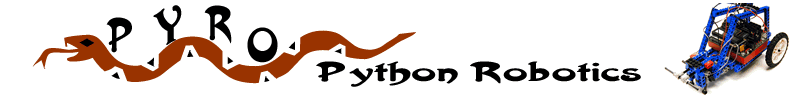
\includegraphics[width=\linewidth]{figs/PyroLogo-0.png}\\
 	   \column{.15\textwidth}
	\end{columns}
\end{frame}

\begin{frame}{Introduction (III)}
    \begin{columns}
 	   \column{.2\textwidth}
		Simulation

 	 	\begin{itemize}
		\item Gazebo
        \item STDR
        \item V-Rep
        \item Stage
		\item MORSE
		\item Webots
        \item[] \href{https://www.youtube.com/watch?v=0uifKcF0TRU}{(Video)}
		\end{itemize}


 	   \column{.4\textwidth}
        \begin{tabular}{cc}
            
\includegraphics[width=0.2\linewidth]{figs/gazebo.png}&
            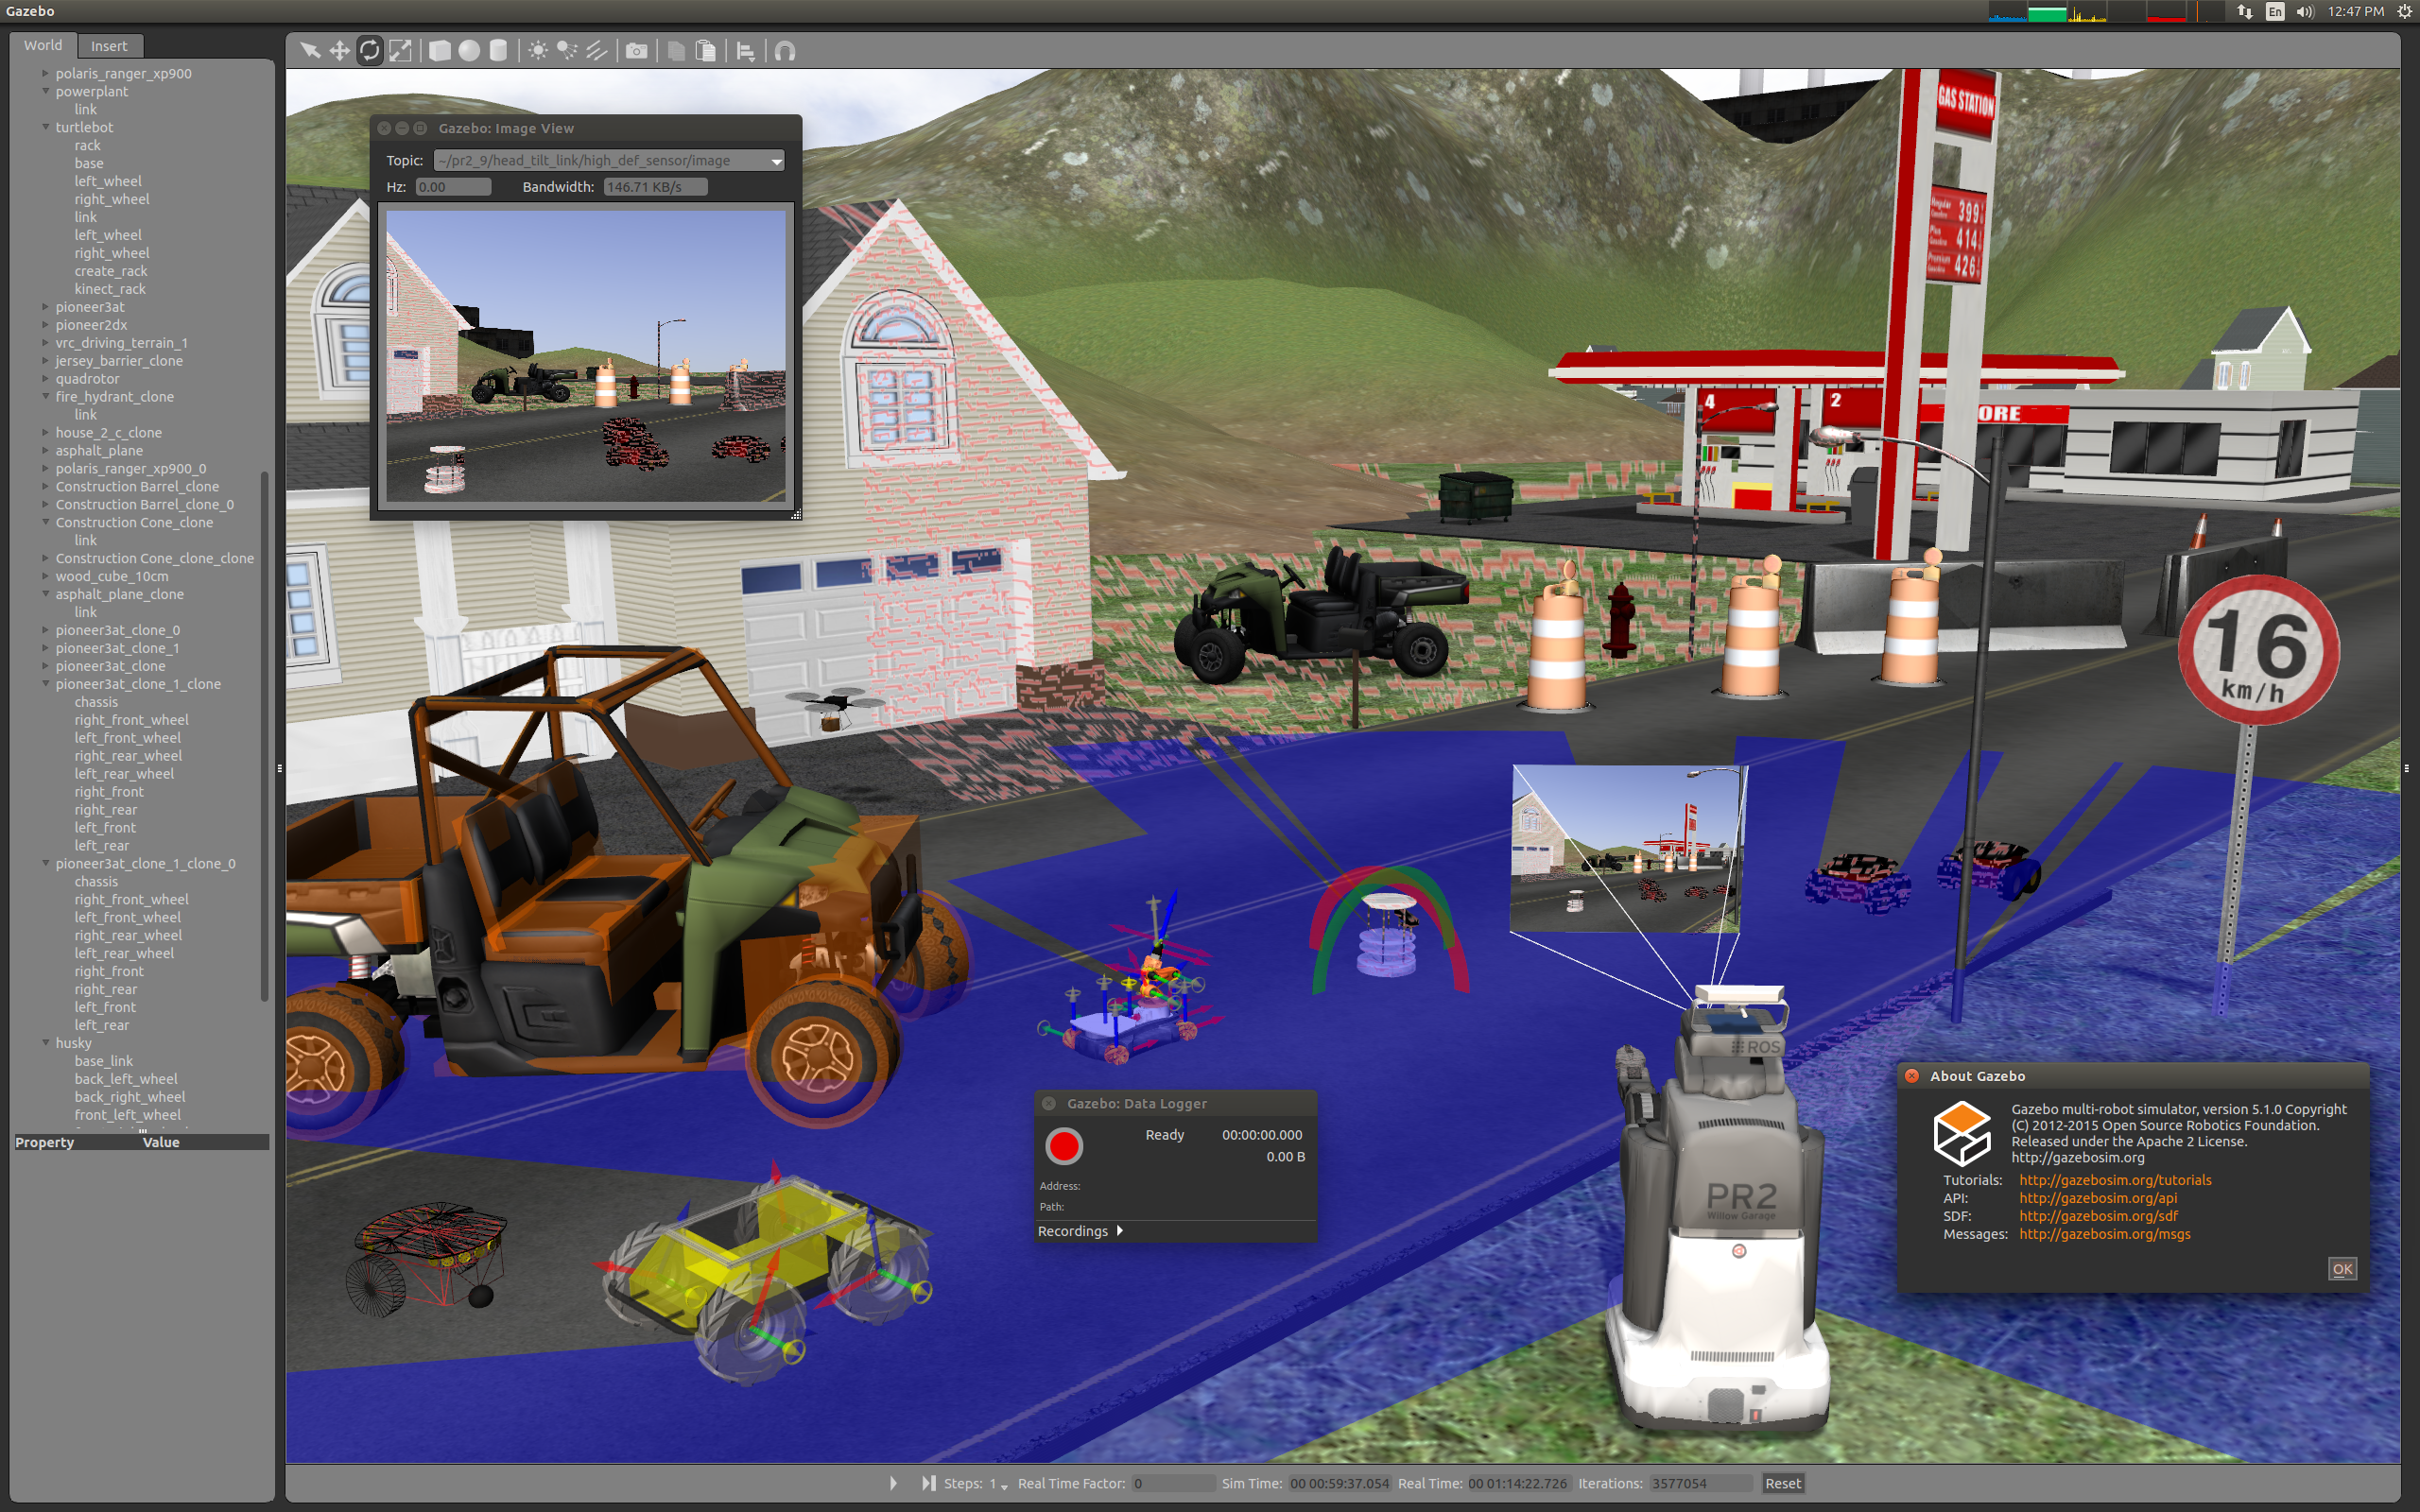
\includegraphics[width=0.6\linewidth]{figs/gazeboScreen.png} \\
            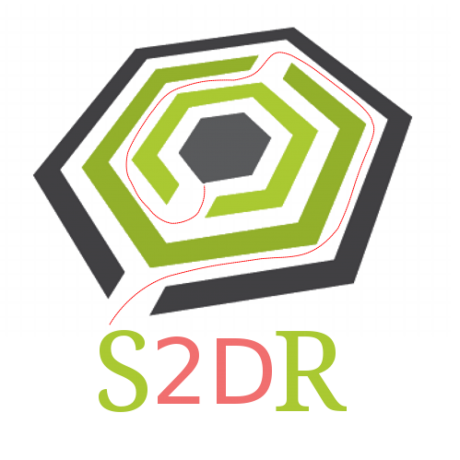
\includegraphics[width=0.3\linewidth]{figs/stdr.png}&
            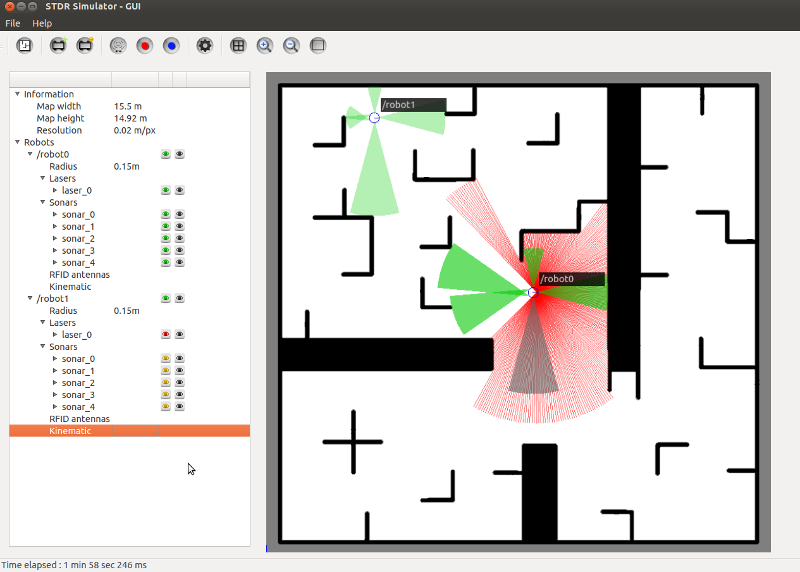
\includegraphics[width=0.6\linewidth]{figs/stdrScreen.png} \\
            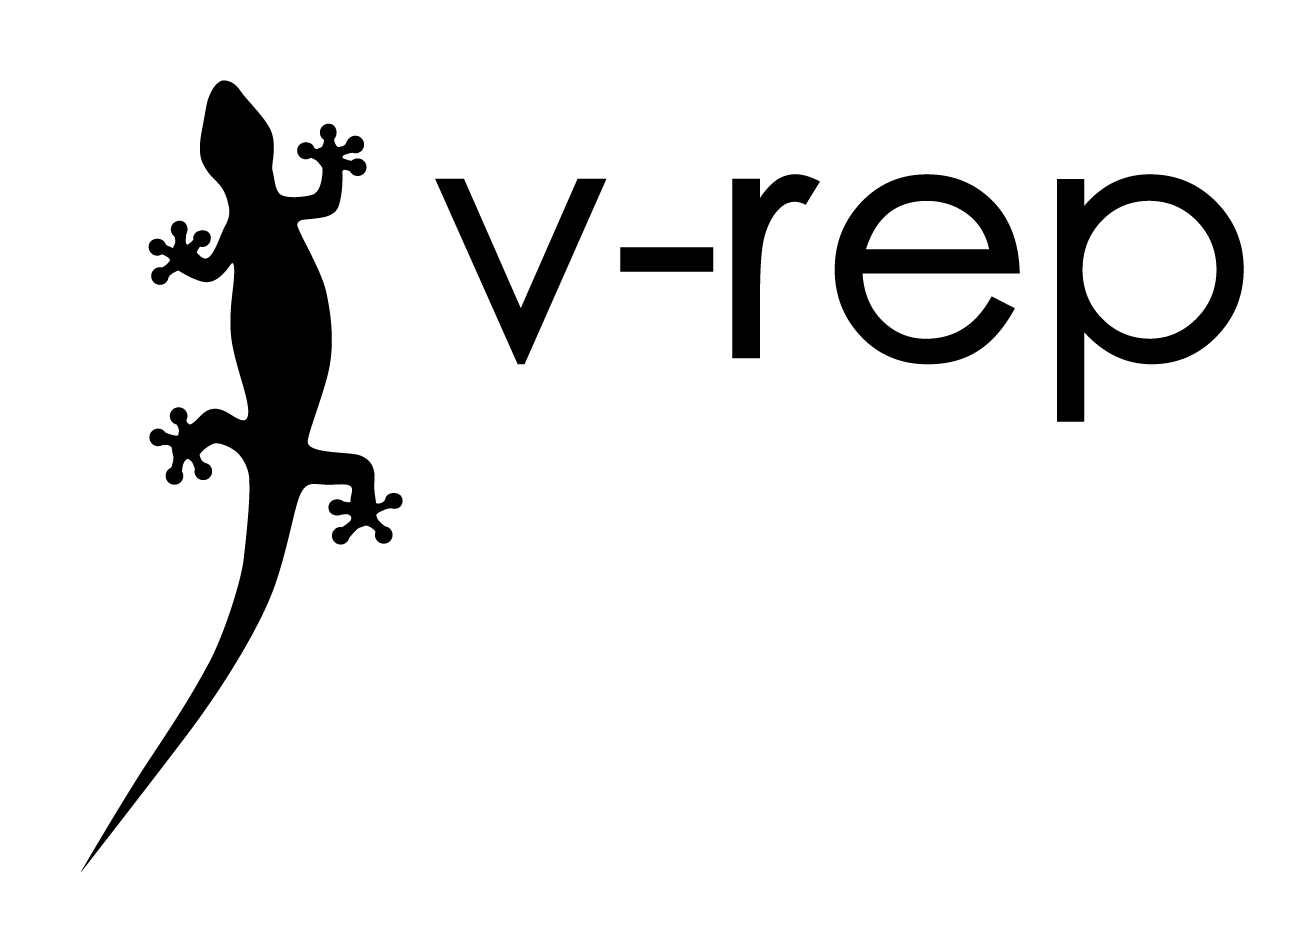
\includegraphics[width=0.3\linewidth]{figs/vrep.png}&
            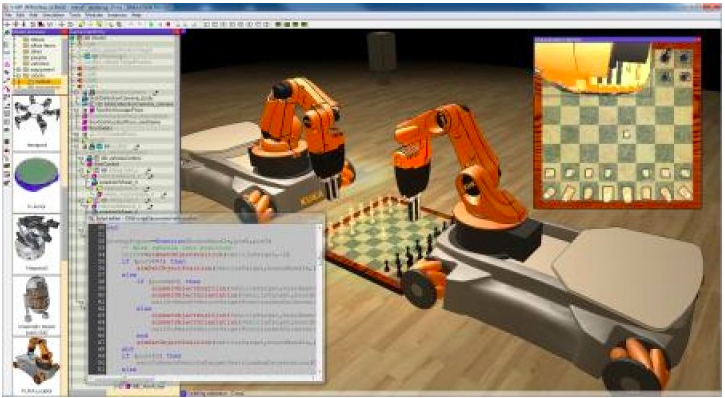
\includegraphics[width=0.6\linewidth]{figs/vrepScreen.png} \\
        \end{tabular}
        \column{.4\textwidth}
        \begin{tabular}{cc}
            
\includegraphics[width=0.3\linewidth]{figs/stage.png}&
            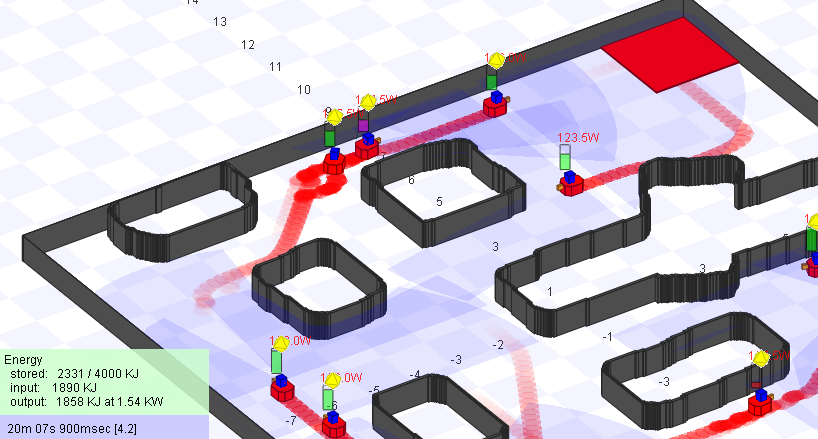
\includegraphics[width=0.6\linewidth]{figs/stageScreen.png} \\
            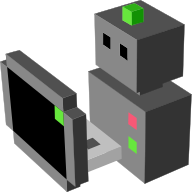
\includegraphics[width=0.2\linewidth]{figs/morse-logo.png}&
            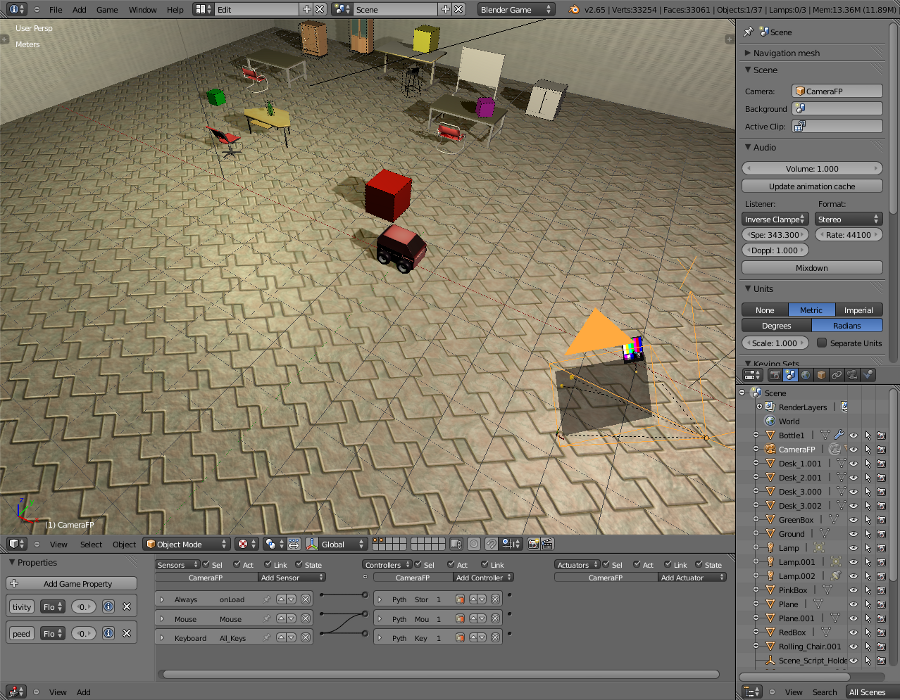
\includegraphics[width=0.6\linewidth]{figs/morseScreen.png} \\
            
\includegraphics[width=0.2\linewidth]{figs/webots.png}&
            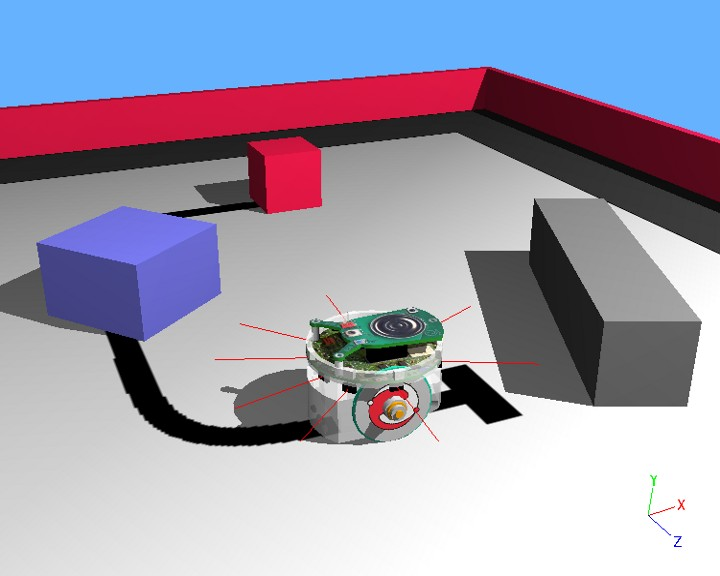
\includegraphics[width=0.6\linewidth]{figs/webotsScreen.png} \\
        \end{tabular}
	\end{columns}
    \bigskip
	\centering Problem: Perception visualization
\end{frame}

\begin{frame}{Introduction (IV)}
    \begin{columns}
 	   \column{.10\textwidth}
 	   \column{.25\textwidth}
		Sensor visualization
 	 	\begin{itemize}
		\item RViz
		\end{itemize}

		Complex motion
 	 	\begin{itemize}
		\item MoveIt!
		\end{itemize}

        \href{https://youtu.be/i--Sd4xH9ZE}{(Video)}

 	   \column{.60\textwidth}
		\centering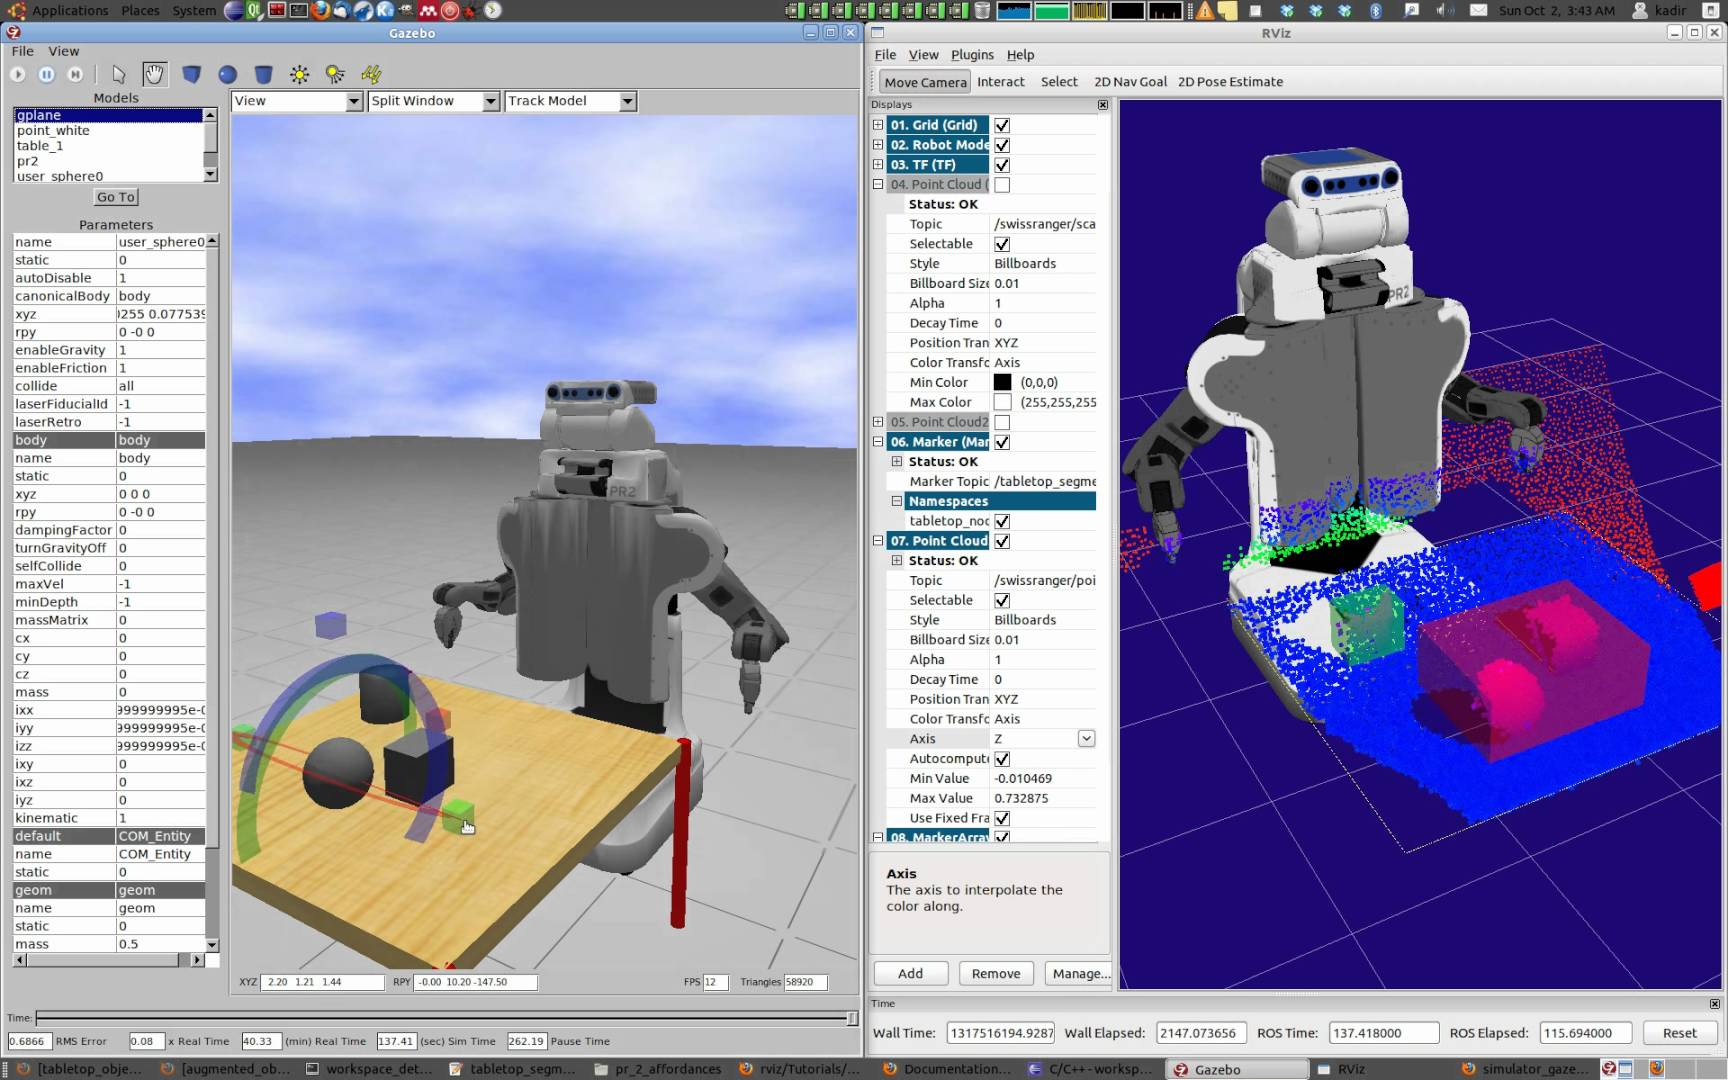
\includegraphics[width=\linewidth]{figs/rosgazebo.jpg}\\
 	   \column{.10\textwidth}
	\end{columns}
\end{frame}

\begin{frame}{Introduction (V)}
	\begin{columns}
 	   \column{.70\textwidth}
	 	\begin{block}{The robot developer toolkit}
		\begin{itemize}
		\item Robot
		\item Linux $\Rightarrow$ Operating system
		\item ROS $\Rightarrow$ Robotic platform
		\item Gazebo $\Rightarrow$ Simulator
		\item RViz $\Rightarrow$ Sensor visualization
		\item MoveIt! $\Rightarrow$ Motion operation
		\end{itemize}
	\end{block}
	\end{columns}
		%\centering
\includegraphics[width=10px]{figs/ros.png}
		%
\includegraphics[width=10px]{figs/gazebo.png}
		%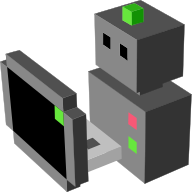
\includegraphics[width=10px]{figs/morse-logo.png}
\end{frame}

\section{Robot Operating System (ROS)}
\begin{frame}{Robot Operating System (ROS) (I)}
\begin{center}
	
\includegraphics[width=0.25\linewidth]{figs/ros.png}\\
\end{center}
	ROS is an ``operating system'' for robots 
	\begin{itemize}
		\item Actually, despite its name, ROS is not an operating system
		\item Located on the operating system and under the applications
		\item ROS is a \textit{robotic platform}
	\end{itemize}
	ROS was created in the Standford AI Lab, in 2007
	\begin{itemize}
		\item Continuous development since then
		\item Almost a standard in research
		\item Increasing popularity in the industry
	\end{itemize}
\end{frame}

\begin{frame}{Robot Operating System (ROS) (II)}
	ROS provides
	\begin{itemize}
		\item An execution environment
		\item A computation model (robot abstraction)
		\item Tools (like RViz and MoveIt!)
		\item Hardware independence
	\end{itemize}

	Features
	\begin{itemize}
		\item Robot drivers
		\item Advanced algorithms (SLAM, navigation, etc)
		\item Large number of supported sensors
		\item Pose estimation, localization, and navigation
		\item Standard robot messages
	\end{itemize}
\end{frame}

\section{ROS versions}
\begin{frame}[plain]{ROS versions}

	\begin{tabular}{llcl}
	\textbf{Version}& \textbf{Release} & \textbf{Logo}\\
	Lunar Loggerhead& May 23rd, 2017   & 
\includegraphics[width=0.08\linewidth]{figs/lunar.png}&\\
	Kinetic Kame	& May 23rd, 2016   & 
\includegraphics[width=0.08\linewidth]{figs/kinetic.png}&\\
	Jade Turtle		& May 23rd, 2015   & 
\includegraphics[width=0.08\linewidth]{figs/jade.png}&\\
	Indigo Igloo 	& July 22nd, 2014  & 
\includegraphics[width=0.08\linewidth]{figs/indigo.png}&Stable\\
	Hydro Medusa 	& Sept. 4th, 2013 & 
\includegraphics[width=0.08\linewidth]{figs/hydro.png}&\\
	Groovy Galapagos& Dec. 31, 2012   & 
\includegraphics[width=0.08\linewidth]{figs/groovy.jpg}&\\
	Fuerte Turtle	& April 23, 2012   & 
\includegraphics[width=0.08\linewidth]{figs/fuerte.jpg}&\\
	Electric Emys	& August 30, 2011   & 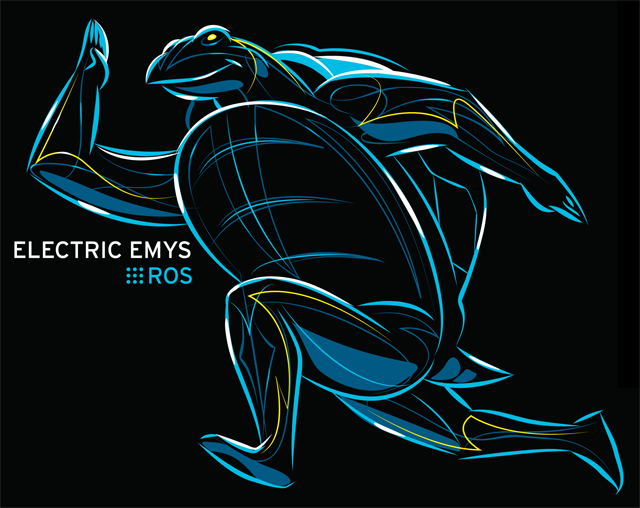
\includegraphics[width=0.08\linewidth]{figs/electric.png}&\\
	\end{tabular}
	\begin{center}
	Significant differences among versions!
	\end{center}
\end{frame}

\section{Installation}
\begin{frame}{Installation}
		ROS runs over Linux
			\begin{itemize}
				\item Ubuntu recommended (official packages available)
				\item Ubuntu and ROS version strongly coupled
				\item Any Linux machine supports, in theory, ROS
				\item Warning: Installing ROS on weird platforms hurts!
			\end{itemize}
		Detailed installation instructions available
			\begin{itemize}
				\item \url{http://wiki.ros.org/jade/installation/}
			\end{itemize}
		We will use a VM with ROS installed in advance (you're welcome :)
\end{frame}

\section{Documentation}
\begin{frame}{Documentation}
	\begin{itemize}
		\item All the ROS documentation is available on its \href{http://wiki.ros.org/}{wiki}
		\item \href{http://wiki.ros.org/ROS/Tutorials}{ROS tutorials} are a good entry point to ROS
		\item Be careful with ROS version
		\item Each robot is coded in a package, each package has its own documentation
	\end{itemize}
\end{frame}

%\section{Exercises}
\begin{frame}{Exercises}{Environment setup}
	\begin{enumerate}
		\item Install VM with ROS Indigo
			\begin{itemize}
			\item VM image in \url{http://nootrix.com/software/ros-indigo-virtual-machine/}
			\item User: \texttt{viki}, password: \texttt{viki}
			\end{itemize}
		\item Configure Spanish keyboard in the VM
		\item Set up the display resolution in the VM
		\item Update packages in the VM (do not jump this step!)
		\item Install ROS Turtlebot packages
			\begin{itemize}
			\item \texttt{apt-get install ros-indigo-turtlebot-*}
			\item \texttt{apt-get install ros-indigo-robot-state-publisher}
			%\item \texttt{apt-get install ros-indigo-turtlebot-gazebo ros-indigo-turtlebot-teleop ros-indigo-turtlebot-rviz-launchers}
			\item Close terminal (important!)
			\end{itemize}
	\end{enumerate}
\end{frame}

\begin{frame}{Exercises}{Basic rover: TurtleBot}
	\begin{columns}
 	   \column{.60\textwidth}
	\begin{enumerate}
		\item Run Gazebo simulation
			\begin{itemize}
			\item \texttt{roslaunch turtlebot\_gazebo turtlebot\_world.launch}
			\end{itemize}
	\item Run Turtlebot teleoperation
			\begin{itemize}
			\item \texttt{roslaunch turtlebot\_teleop keyboard\_teleop.launch}
			\end{itemize}
	\item Run RViz real-time data visualization 
			\begin{itemize}
			\item \texttt{roslaunch turtlebot\_rviz\_launchers view\_robot.launch}
			\end{itemize}
	\end{enumerate}

 	   \column{.40\textwidth}
		\centering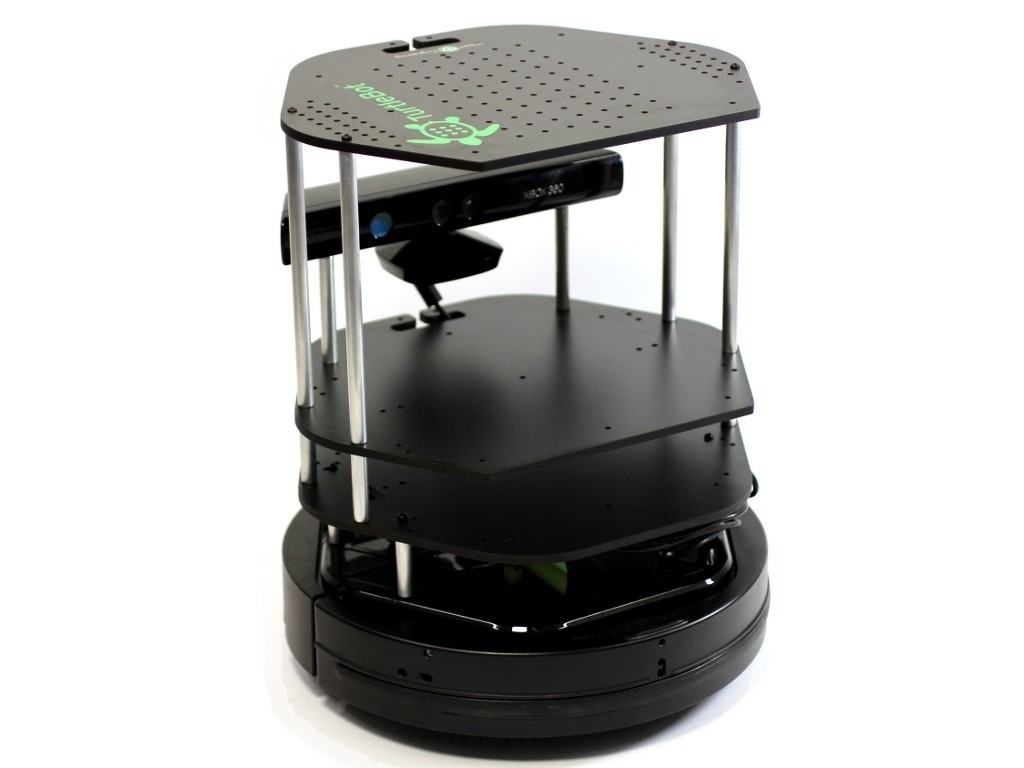
\includegraphics[width=\linewidth]{figs/turtlebot.jpg}
	\end{columns}
\end{frame}

%\begin{frame}{Exercises}{Basic rover: SLAM with TurtleBot}
%	\begin{columns}
% 	   \column{.60\textwidth}
%	\begin{enumerate}
%		\item Install SLAM libraries
%			\begin{itemize}
%			\item \texttt{sudo apt-get install ros-indigo-slam-gmapping}
%			\end{itemize}
%	\item Run simulation with SLAM
%			\begin{itemize}
%			\item \texttt{roslaunch turtlebot\_navigation gmapping\_demo.launch}
%			\end{itemize}
%	\item Run teleoperation
%			\begin{itemize}
%			\item \texttt{roslaunch turtlebot\_teleop keyboard\_teleop.launch}
%			\end{itemize}
%	\end{enumerate}

% 	   \column{.40\textwidth}
%		\centering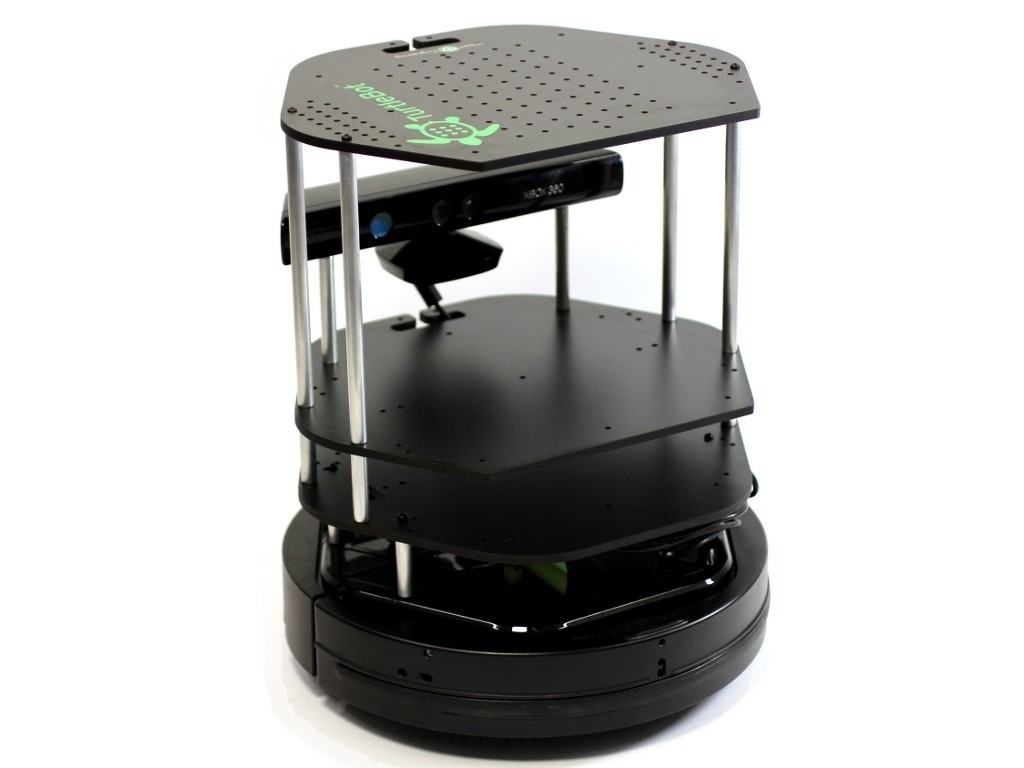
\includegraphics[width=\linewidth]{figs/turtlebot.jpg}
%	\end{columns}
%\end{frame}

\begin{frame}{Exercises}{Mobile manipulator: PR2}
	\begin{columns}
 	   \column{.70\textwidth}
		\begin{enumerate}
		\item Install PR2 and Moveit!
			\begin{itemize}
			\item \texttt{sudo apt-get install ros-indigo-moveit-pr2 ros-indigo-moveit-ros-visualization}
			\item Close the terminal and open a new one
			\end{itemize}
		\item Run RViz and Moveit
			\begin{itemize}
			\item \texttt{roslaunch pr2\_moveit\_config demo.launch}
			\end{itemize}
		\end{enumerate}
 	   \column{.30\textwidth}
		\centering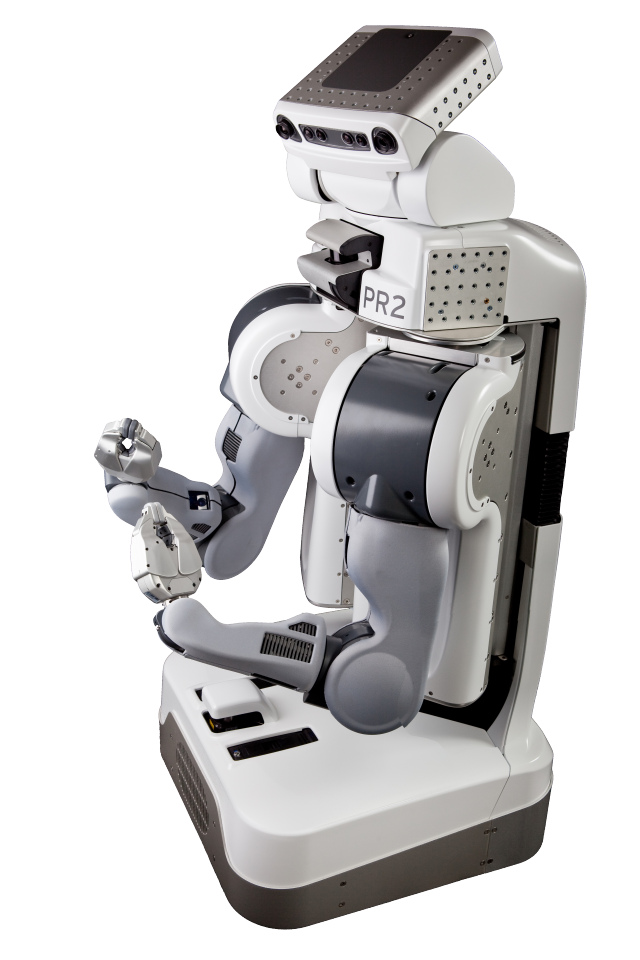
\includegraphics[width=0.9\linewidth]{figs/pr2.jpg}
	\end{columns}
\end{frame}

\begin{frame}{Exercises}{UAV: Hector quadrotor}
	\begin{columns}
 	   \column{.70\textwidth}
	\begin{enumerate}
		\item Install Hector quadrotor: 
			\begin{itemize}
			\item \texttt{sudo apt-get install ros-indigo-hector-*}
			%\item \texttt{sudo apt-get install ros-indigo-hector-quadrotor-gazebo}
			\item Close the terminal and open a new one
			\end{itemize}
		\item Run simulation
			\begin{itemize}
			\item \texttt{roslaunch hector\_quadrotor\_demo outdoor\_flight\_gazebo.launch}
			\end{itemize}
		\item Run teleoperation (with joystick)
			\begin{itemize}
			\item \texttt{roslaunch hector\_quadrotor\_teleop xbox\_controller.launch}
			\end{itemize}
	\end{enumerate}
 	   \column{.30\textwidth}
		\centering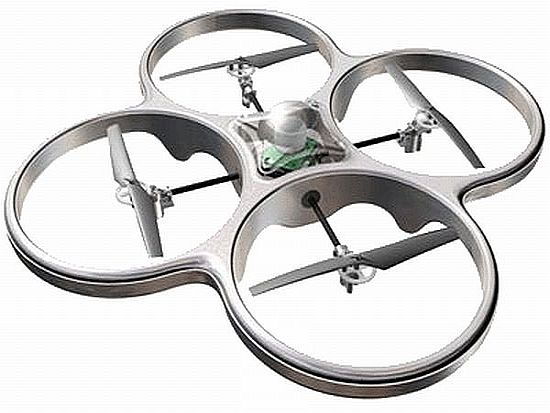
\includegraphics[width=\linewidth]{figs/quad.jpg}
	\end{columns}
\end{frame}

\begin{frame}{Exercises}{UAV: Hector quadrotor (indoor SLAM)}
	\begin{enumerate}
		\item Run simulation
			\begin{itemize}
			\item \texttt{roslaunch hector\_quadrotor\_demo indoor\_slam\_gazebo.launch}
			\end{itemize}
		\item Run teleoperation (with joystick)
			\begin{itemize}
			\item \texttt{roslaunch hector\_quadrotor\_teleop xbox\_controller.launch}
			\end{itemize}
	\end{enumerate}
\end{frame}

\begin{frame}{Exercises}{Humanoid: Nao}
	\begin{columns}
 	   \column{.70\textwidth}
	\begin{enumerate}
		\item Install Nao packages
		\begin{itemize}
		\item \texttt{sudo apt-get install ros-indigo-nao*}
		\end{itemize}
	\item Run Nao demo
		\begin{itemize}
		\item \texttt{roslaunch nao\_gazebo\_plugin nao\_gazebo\_plugin\_H25.launch}
		\end{itemize}
	\item Move robot with Moveit
		\begin{itemize}
		\item \texttt{roslaunch nao\_moveit\_config moveit\_planner.launch}
		\end{itemize}
	\end{enumerate}
 	   \column{.30\textwidth}
		\centering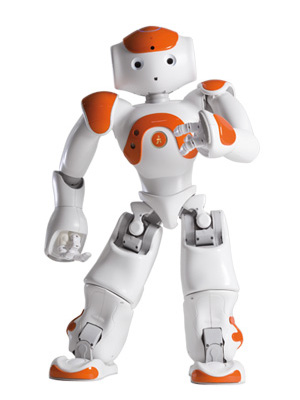
\includegraphics[width=\linewidth]{figs/nao.jpeg}
	\end{columns}
\end{frame}


\end{document}
